\documentclass[12pt]{article}
\usepackage[top=1in,left=1in, right = 1in, footskip=1in]{geometry}

\usepackage{graphicx}
%\usepackage{adjustbox}

\newcommand{\eref}[1]{(\ref{eq:#1})}
\newcommand{\fref}[1]{Fig.~\ref{fig:#1}}
\newcommand{\Fref}[1]{Fig.~\ref{fig:#1}}
\newcommand{\sref}[1]{Sec.~\ref{#1}}
\newcommand{\frange}[2]{Fig.~\ref{fig:#1}--\ref{fig:#2}}
\newcommand{\tref}[1]{Table~\ref{tab:#1}}
\newcommand{\tlab}[1]{\label{tab:#1}}
\newcommand{\seminar}{SE\mbox{$^m$}I\mbox{$^n$}R}

\usepackage{amsthm}
\usepackage{amsmath}
\usepackage{amssymb}
\usepackage{amsfonts}

\usepackage{lineno}
%\linenumbers

\usepackage[pdfencoding=auto, psdextra]{hyperref}

\bibliographystyle{chicago}
\usepackage{natbib}
\date{\today}

\usepackage{xspace}
\newcommand*{\ie}{i.e.\@\xspace}

\usepackage{color}

\newcommand{\Rx}[1]{\ensuremath{{\mathcal R}_{#1}}} 
\newcommand{\Ro}{\Rx{0}}
\newcommand{\RR}{\ensuremath{{\mathcal R}}}
\newcommand{\Rhat}{\ensuremath{{\hat\RR}}}
\newcommand{\tsub}[2]{#1_{{\textrm{\tiny #2}}}}

\newcommand{\comment}[3]{\textcolor{#1}{\textbf{[#2: }\textsl{#3}\textbf{]}}}
\newcommand{\jd}[1]{\comment{cyan}{JD}{#1}}
\newcommand{\swp}[1]{\comment{magenta}{SWP}{#1}}
\newcommand{\dc}[1]{\comment{blue}{DC}{#1}}
\newcommand{\hotcomment}[1]{\comment{red}{HOT}{#1}}

\newcommand{\jdnew}{\jd{NEW}}
\newcommand{\jddel}[1]{\jd{DELETE: #1}}

\begin{document}

\begin{flushleft}{
	\Large
	\textbf\newline{
		Modeling the spread of SARS-CoV-2 on a university campus: lessons from Princeton University
	}
}
\newline
\\ 

\end{flushleft} 

\pagebreak

Predicting and controlling the spread of SARS-CoV-2 remains a critical public health and scientific question.
Rapid, asymptomatic transmission of SARS-CoV-2 has hindered intervention efforts such as contact tracing.
Stringent measures to limit social contacts has been effective in preventing transmission but are unsustainable.
The recent development of vaccines have provided a safe means of reopening the society, but uncertainty remains in their long-term effectiveness as well as .
In addition, as new variants continues to emerge and 

the emergence of new variants, which can evade immunity and transmit better, continues to pose additional challenges.


Since the beginning of the pandemic, mathematical models have played a key role in evaluating intervention measures and guiding pandemic respones.



testing has played a key role in monitoring and controlling the spread.
In addition, a frequent testing of a large fraction of the population, followed by rapid isolation and contact tracing, has proven effective in preventing chains of transmission and reducing the spread in large congregate settings.

University campuses provide unique test case in a relatively well-controlled setting for evaluating the feasibility of safe reopening.
High density environemtns and large fraction of asymptomatic infections (due to young age of university students) can readily permit rapid transmission.

.


- Usual pandemic start

- modeling, understanding control
- testing frequency is important
- universities provide a particularly test case; asymptomatic infection and testing is very high

- little review of what other universities have done

- epideimc in relatively well controlled documented setting
- really well until omicron
- perhaps because of immunity waning 


In this study, we analyze the spread of SARS-CoV-2 on Princeton University campus (\fref{princeton}).
Princeton University is located in Mercer County, New Jersey, USA and consists of roughly 5000 undergraduate students, 3000 graduate students, and 7000 staffs and faculties.
For simplicity, we divide the epidemic into three time periods representing three semesters: Fall 2020 (August 24, 2020--January 1, 2021; \fref{princeton}A), Spring 2020 (January 16, 2021--May 14, 2021; \fref{princeton}B), and Fall 2021 (August 14, 2021--December 24, 2021; \fref{princeton}C).
Throughout the study period, all students, staff and faculty members who were physically present for more than 8 hours on campus per week were required to participate in asymptomatic testing with varying frequencies.
Asymptomatic individuals submitted self-collected saliva samples, from which the presence of SARS-CoV-2 was tested using Polymerase Chain Reaction (PCR) \swp{regular PCR? RT-PCR? what are we using?}.  
Asymptomatic individuals who tested positive were required to isolate for 10 days.
Symptomatic individuals were eligible for rapid PCR tests and had to isolate \swp{self-isolate?} until they received their test results---those who tested positive were required to isolate for at least 10 days after symptom onset ond were release 3 days after symptoms resolved.
Throughout the study period, contact tracing was also performed to quarantine close contacts of confirmed cases.
Close contacts are defined as those who spent \swp{???}.


\begin{figure}[!th]
\includegraphics[width=\textwidth]{../figure_princeton/figure_princeton.pdf}
\caption{
\textbf{Dynamics of SARS-CoV-2 outbreaks in Princeton University}
(A--C) Epidemic trajectories across three semesters: Fall 2020 (A), Spring 2020 (B), and Fall 20201 (C).
Colored bar plots represent the weekly number of cases from both asymptomatic and symptomatic testing in Princeton University.
Red lines represent the weekly number of cases in Mercer County.
Number of cases in Mercery County is obtained from \url{https://github.com/nytimes/covid-19-data}.
(D--F) Correlations between the weekly number of cases in Princeton University and in Mercer County.
Solid lines and shaded areas represent the estimated lienar regression lines and the associated 95\% CIs.
\label{fig:princeton}
}
\end{figure}

During fall 2020, roughly 1000 grad students and 2000 staffs and faculties were present on campus and were subject to asymptomatic testing. 
Undergraduate students were not allowed to return back to campus, and so their numbers were minimal (<300).  
Both undergraduate students and graduate students were required to get tested twice a week, whereas staffs and faculties were required to get tested once a week.
The number of cases remained relatively low throughout the semester with peak occuring in early December, coinciding with the epidemic trajectory in Mercer County (\fref{princeton}A).
We note that a sudden decrease in the number of cases around Thanksgiving may reflect reduced number of tests (3852 and 2972 asymptomatic tests performed on the week ending November 20th and 27th, respectively) as well as actual transmission.
The highest number of cases was reported among staffs and faculties (169), followed by graduate students (41), and undergraduate students (4).

In the beginning of spring 2020, the number of cases suddenly increased before classes began (\fref{princeton}B), reflecting $\approx 3000$ undergraduate students returning to campus and bringing back infections.
Returning students were required to be tested and quarantine \swp{for how long} if they were coming back from CDC-designated states \swp{not sure if this is the right wording... but I remember we had a rule like this...}.
The classes remained virtual and testing protocol did not change (twice a week for undergraduate and graduate students, and once a week for staffs and faculties).
The number of cases persisted at similar levels as the fall semester and eventually decreased as classes ended and students went back home---the decrease in the number of cases in Princeton University also coincided with the decrease in the number of cases in Mercer County.
The highest number of cases was reported among staffs and faculties (111), followed by undergraduate students (101), and graduate students (29).

In fall 2021, all students, staffs, and faculties were required to be vaccinated \swp{with two doses?} with a very few exceptions for medical and religious reasons. 
By the beginning of the semesters, ??\% of students and ??\% of staffs and faculties were vaccinated.
As of January 11th, 99\% of undergraduate students, 98\% of graduate students, and 96\% of staffs and faculties have been vaccinated.
Vaccinated individuals were required to be tested once a week, while unvaccinated individuals were required to be tested twice a week.
In-person teaching and activities were allowed on campus.
Everyone was required to wear masks indoors with a few exceptions (e.g., when eating or drinking, or when teaching a small class).
The number of cases remained similar to previous semesters until November when the number of cases began to increase primarily among undergraduate students around Thanksgiving (\fref{princeton}C).  
On November 27th, 2021, Princeton University announced undergraduate students to be tested twice a week and limited the size of non-academic gatherings to 20 people.
The number of cases decreased slightly as classes ended but soon increased back up as the Omicron variant was introduced on campus as well as in Mercer County.

Across all three semesters, we find strong and significant correlations between the weekly logged numbers of cases from Princeton University and those from Mercer County:
Fall 2020 ($\rho = 0.81$  (95\% CI: 0.55--0.92); $p < 0.001$; \fref{princeton}D); Spring 2020 ($\rho = 0.80$  (95\% CI: 0.51--0.92); $p < 0.001$; \fref{princeton}E); and Fall 2021 ($\rho = 0.90$  (95\% CI: 0.78--0.96); $p < 0.001$; \fref{princeton}F). 
Although we cannot infer causation from correlations, these strong correlations are likely indicative of community imports driving epidemic patterns on campus.
Indeed, contact tracing analyses suggest that the majority of cases were linked with community transmission until fall 2021 when transmission clusters were identified on campus (e.g., holiday parties). \swp{Can we provide more quantitiative information than this? Or is IRB going to hate us?}

\section*{Mathematical model}

We use a discrete-time, individual-based model to simulate the spread of SARS-CoV-2 in Princeton University and to evaluate effects of intervention measures, such as testing.
The model consists of five main components that are simulated on a daily time scale: (1) transmission and infection dynamics, (2) sampling and testing protocols, (3) contact tracing, (4) quarantine and isolation protocols, and (5) vaccination dynamics, including waning immunity and booster shots.
Here, we describe each component briefly (see Supplementary files for details).

Infection processes are modeled based on standard compartmental models.
Once infected, susceptible individuals enter the exposed stage, during which they cannot transmit or test positive. 
After $D_e$ days on average, exposed individuals then enter the presymptomatic, during which they can test positive and transmit infections at rate $\beta_p$ for $D_p$ days on average.
Presymptomatic individuals can then either remain asymptomatic with probability $p_a$ or develop symptoms with the remaining probability of $1-p_a$; both asymptomatic and symptomatic individuals are assumed to have the same duration of infection ($D_s$) and transmission rates ($\beta_s$) for simplicity.
Recovered individuals are assumed to be immune to reinfections throughout a semester.
Transmissions are modeled using a negative binomial distribution with an overdispersion parameter of $k=0.1$ to account for the possibility of super-spreading events.
External (community) transmission is modeled using a Poisson distribution with a time-varying mean calculated by scaling the daily number of cases by $\theta$ and shifting it by 1 week to account for reporting delays.

All individuals on campus are assumed follow a pre-determined asymptomatic testing plan at a fixed frequency for simplicity---
for example, under weekly testing, one individual can get sampled on days 1, 8, and 15, whereas another inidividual get sampled on days 2, 9, and 16.
We assume that test results come back after one day.
Symptomatic individuals can choose to take rapid PCR tests (with results returning on the same day) with a given probability on each day until their symptoms resolve---this probability is set to 1 for simulations presented in the main text.
We further assume that symptomatic individuals would isolate immediately when they submit their samples until they receive negative results.
All individuals who test positive are required to isolate (following the same isolation rule as before) and are exempt from asymptomatic testing for 90 days.
Isolated individuals are assuemd to no longer transmit infections.
We assume that PCR tests have 95\% sensitivity and 100\% specificity.

When an individual tests positive, contact tracing is performed to identify and quarantine their contacts.
Contact tracing depend on two parameter: tracing efficacy, which we define as the proportion of secondary infections, and tracing delay, which represents the time between when an individual tests positive and when their contacts are quarantined.
Following Princeton \swp{New Jersey? CDC?} guidelines for contact tracing, contacts are traced up to two days before symptom onset or two days before the positive test (for asymptomatic cases).
Quarantined individuals are released after 14 days.
We do not model quarantining of non-infectious contacts as they do not affect epidemic dynamics.
For simplicity, we do not model contact tracing during parameter matching.

As most students, staffs, and faculties had received two doses of vaccination in the beginning of fall 2021, we do not distinguish the first and second doses.
Instead, we assume that vaccines reduce susceptibility as well as transmissibility of all vaccinated individuals by an equal amount for all vaccinated individuals.
Vaccine efficacies against both infection and transmission are allowed to exponentially wane from 90\% to 50\% in 20 weeks (and continues to wane at the same rate) for each vaccinated individuals.

This model was developed and used throughout the pandemic to inform policy decisions in Princeton University, including the frequency of asymptomatic tests and the number of isolation beds required.
We continuously updated the model to reflect changes in school settings (e.g., students returning back to campus in spring 2020) as well as intervention measures (e.g., vaccination in fall 2021 and booster shots with the emergence of the Omicron variant).
The model we use here is a generic version that encompasses all of the necessary details to model the spread of SARS-CoV-2 in Princeton University.
Here, we use this model to retrospectively analyze past outbreaks and further predict what future epidemic trajectories might look like as the new Omicron variant spreads on campus.
Simulation details are provided in the supplementary materials.

First, we try to match our model to epidemic patterns seen on campus by varying the basic reprodcution number $\mathcal R_0$ and the amount of community transmission $\theta$ and holding all other parameters constant.
For each parameter combination, we simulate 100 epidemic trajectories and calculate the sum of squared differences between the weekly numbers of the observed and predicted positive cases.
The population size and testing frequencies (with twice weekly testing modeled as testing every 3 days) are set to previously discussed values to reflect realistic campus settings.


\begin{figure}[!th]
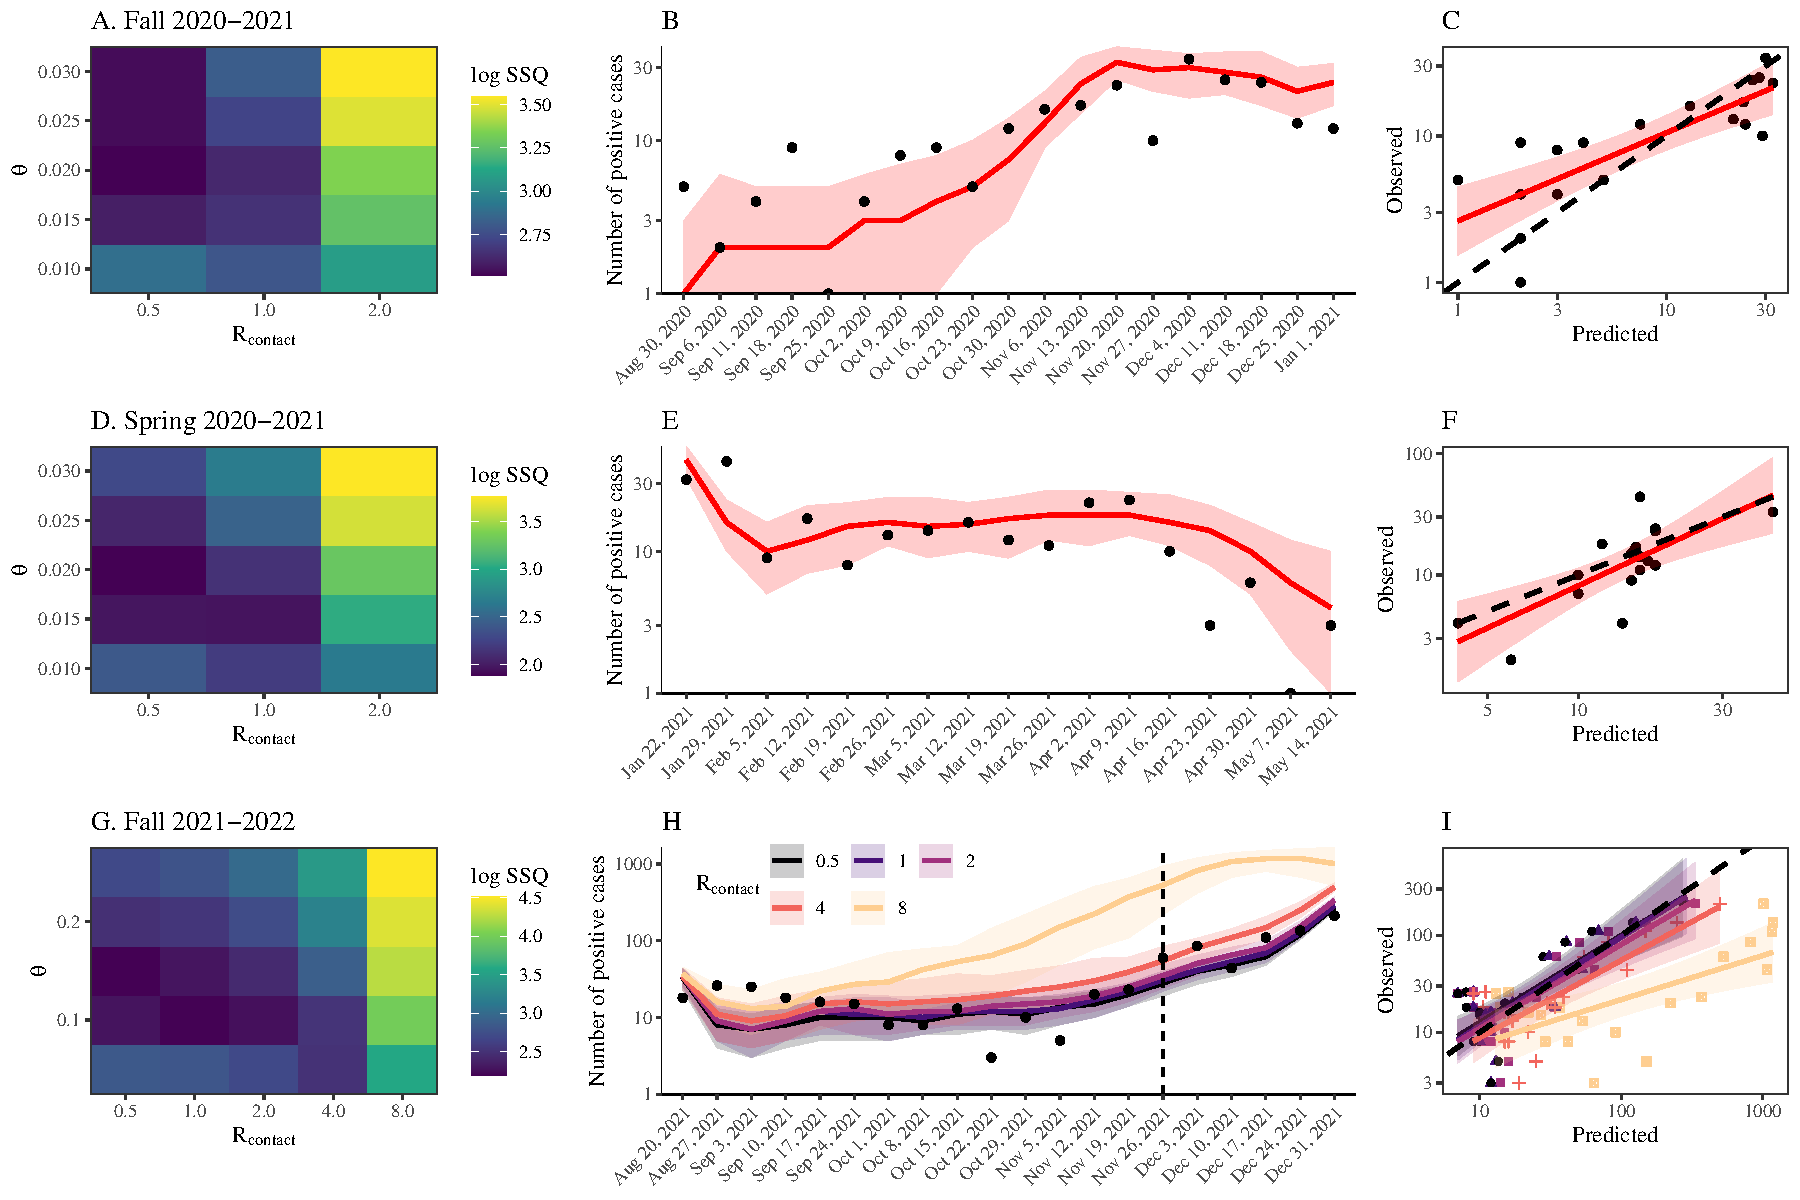
\includegraphics[width=\textwidth]{../figure_princeton/figure_princeton_simulation.pdf}
\caption{
\textbf{Dynamics of SARS-CoV-2 outbreaks in Princeton University}
(A, D, G) Time series comparisons of model predictions with observed data across ranges of paramters: basic reproduction number $\mathcal R_0$, scaling parameter for community transmission $\theta$, and the initial proportion of infected individuals $I_0$.
For each paramter combination, we simulate the model 100 times and calculate the sum of squared differences (SSQ) between the reported number of positive cases and the model-predicted number of positive cases. 
Heatmaps represent medians of the logged sum of squared differences.
(B, E, H) Model predictions. 
Solid lines represent median predictions.
Shaded areas represent 90\% quantiles for the best matching parameter set.
Points represent the observed data.
(C, F, I) Correlations between model predictions with observed data.
Colored solid lines and shaded areas represent the estimated lienar regression lines and the associated 95\% CIs.
Dashed lines represent the one-to-one line.
\label{fig:matching}
}
\end{figure}


We find that a low value of $\mathcal R_0=0.5$ and a small amount of community transmission $\theta=0.015$ is most consistent with the observed epidemic dynamics in fall 2020 (\fref{matching}A).
With these parameters, the model is able to capture the rise and fall in the number of cases with the exception of sudden decrease in the number of cases around Thanksgiving, which we do not model explicitly (\fref{matching}B).
The median predictions are positively correlated with the observed dynamics ($\rho = 0.83$; 95\% CI: 0.61--0.93; \fref{matching}C).
Although a wide range of assumptions about the levels of community transmission $\theta$ are consistent with the observed dynamics, our simulations preclude high $\mathcal R_0 > 2$ (SUPP).
Distancing measures on campus, including virtual classes, likely contributed to lowering $\mathcal R_0$.

A similar set of parameters can capture the observed dynamics in spring 2020.
The best matching parameter predicts a slightly higher levels of community transmission $\theta=0.02$ (\fref{matching}D), but a wide range of parameters are consistent with the observed dynamics as before (SUPP). 
Simulations also preclude high $\mathcal R_0 > 2$ again, suggesting that the contact levels between students likely remained low even though they had returned to campus---low $\mathcal R_0$ may be attributed in part to the absence of in-person teaching.
We note that the introduction of infections from returning students are necessary to capture the initial rise in the number of cases (\fref{matching}E).
Once again, we find a positive (but slightly weaker) correlation between the predicted and the observed numbers of cases ($\rho = 0.62$; 95\% CI: 0.20--0.85; \fref{matching}F).

For fall 2021, we limited our model comparison to November 26th before the Omicron variant was introduced on campus.
We assume that $>95\%$ of the school population is vaccinated at the beginning of the semester and do not model additional doses throughout the semester for simplicity.
We also allow vaccine-derived immunity to wane over time to ask whether the increase in the number of cases around November is consistent with the dynamics predicted by immunity waning.

Even though the numbers of cases during fall 2021 (before a large outbreak) were similar to those during previous semesters, we find that considerably higher levels of community transmission $\theta$ (~10 fold higher) is required to explain the observed dynamics due to a decreased susceptibility from vaccination (\fref{matching}G).
We note that the parameter $\theta$ necessarily depends on our assumed vaccine efficacy, and $\theta$ would decrease if we assume a lower vaccine efficacy.
Nonetheless, the amount of community transmission would still need to be higher than previous semesters as long as vaccine provides some protection against infection.

We also find that the predicted dynamics are largely insensitive to $\mathcal R_0$ until November 26th (\fref{matching}H)---
in addition, all simulations shown in \fref{matching}H are positively correlated with the observed numbers of cases (\fref{matching}G). 
An increasing pattern in the sum of squared errors with $\mathcal R_0$ shown in \fref{matching}G is primarily driven by the discrepancy around fall break (week ending October 26th) when the number of cases decreased suddenly, which we do not model explicitly.
As nearly all school population was vaccinated, transmission between individuals on campus would have been limited, making $\mathcal R_0$ difficult to estimate.
These simulations also suggest that an increase in the number of cases in November can be explained by a combination of waning immunity alone without requiring additional changes in transmission dynamics (note we do not allow $\theta$ or $\mathcal R_0$ to vary over time).

Projecting the model beyond November 26th shows that we would have seen a similarly growth in the number of cases if conditions remained constant even without the introduction of the Omicron variant.
In other words, the Delta strain would have continued to spread on campus at a similar rate if the semester were to (hypothetically) continue until January without additional interventions (\fref{matching}H).
In reality, the situation was more complex:  testing frequencies increased and social gatherings were limited in response to an increase in the number of cases.
These interventions---as well as students returning back home as classes ended---likely would have reduced contact rates (and therefore transmission of the Delta variant).
This reduction in transmission was likely counterbalanced by the introduction of the Omicron variant and its immune evasion, leading to similar and persistent growth in the number of cases.

We then project epidemic trajectories for the spread of the Omicron variant among 4000 students for the spring semester of 2021 across a wide range of basic reproduction number ($\mathcal R_0 = 2--16$) and testing frequencies (every 2, 4, and 7 days).
We assume a two-dose efficacy 10\% and a three-dose efficacy of 70\% against the infection and transmission of the Omicron variant. 
We further assume that immunity from the third dose takes 14 days to develop and can wane at the same rate as previously assumed (in this case, 70\% to 39\% in 20 weeks).
For simplicity, we assume a constant amount of external infections.

\fref{omicron} shows predicted trajectories of new infections per day (A) and the mean susceptibility over time (B).
Across a wide range of $\mathcal R_0$, we find that frequent testing alone is not sufficient to prevent an outbreak---while testing and isolation can prevent onward transmission once infected, it cannot prevent infections from happening especially if they are coming from outisde of the population.
Administering booster shots at a faster rate (compare 30 vs 60 booster shots per day in \fref{omicron}A) can help reduce the size of the epidemic peak and cause the epidemic to decay faster, their overall impact is limited due to delays in developing immunity and imperfect protection against the Omicron variant.
Comparing changes in the mean susceptibility further reveal that administering booster shots at a faster rate can also lead to earlier immunity waning and higher mean susceptibility by the end of the semester, which may increase chances of an outbreak in the future \fref{omicron}.

\begin{figure}[!th]
\includegraphics[width=\textwidth]{../figure_omicron/figure_omicron.pdf}
\caption{
\textbf{Scenario projects of the spread of omicron variant on university campus}
(A) The predicted daily number of new infections across a wide ranges assumptions about testing frequencies, basic reproduction number $\mathcal R_0$, and the number of booster shots given per day.
(B) The predicted effective susceptibility over time. 
Effective susceptibility is calculated by taking the mean of individual-level susceptibility of each student.
Solid lines and shaded areas represent the median and the corresponding 90\% quantiles across 100 simulations.
All other parameters are the same as in Figure 2.
\label{fig:omicron}
}
\end{figure}

So far we have assumed that all individuals who test positive are isolated for 10 days;
in practice,  however, isolation of infected individuals can be limited by the isolation bed capacity.
As the Omicron variant to spread rapidly on university campuses (\fref{omicron}), universities participating in testing plans can expect to face difficulties in isolating infected individuals.
Here, we explore how limitintg the number of isolation beds on university campus can affect epidemic dynamics by assuming that individuals who test positive will not be isolated and will continue to transmit when isolation beds are full.
In doing so, we also consider the effects of shorter isolation periods (5, 7, and 10 days).

\begin{figure}[!th]
\includegraphics[width=\textwidth]{../figure_omicron/figure_omicron_limit.pdf}
\caption{
\textbf{Scenario projects of the spread of omicron variant on university campus with limited isolation beds}
(A) The predicted numbers of individuals in isolation on a given day.
(B) The predicted daily number of new infections.
Solid lines and shaded areas represent the median and the corresponding 90\% quantiles across 100 simulations.
We assume $\mathcal R_0 = 8$, 30 booster shots given per day, and testing frequency of 3 days for these simulations.
All other parameters are the same as in Figure 3.
\label{fig:isolation}
}
\end{figure}

When there are no limits to the number of isolation beds on campus, shortening isolation periods results in a slightly higher number of total infections (\fref{isolation}A): .
The epidemic trajectory remains similar across different values of isolation periods (\fref{isolation}B), but the number of students in isolation becomes considerably lower with shorter isolation periods (\fref{isolation}C).
For example, the maximum number of students in isolation decreases from ??? to ???.

When the number of isolation beds is moderately limited ($=200$), shortening isolation periods can decrease the total numbers of infections (\fref{isolation}A) and considerably reduce the size of the epidemic peak (\fref{isolation}B). 
Even when the number of isolation beds is severly limited ($=100$), shortening isolation periods can still reduce the size of the epidemic peak (\fref{isolation}B) because we are able to isolate a greater proportion of infected individuals and prevent onward transmission.
Longer isolation can prevent a greater amount of onward transmission \emph{per individual} but permits a lower number of individuals in isolation, making it less effectivess when the number of isolation beds are limited.

\section{Discussion}

Here, we present the analysis of SARS-CoV-2 outbreaks on Princeton University campus between fall 2020 and winter 2022.
Our analysis demonstrates strong spatiotemporal correlations between the patterns of spread of SARS-CoV-2 on university campus and those from surrounding communities.
These correlations decrease with distance from Mercer County in fall 2021, likely reflecting contact and commuting patterns as university re-opened.
Mathematical modeling further suggests limited transmission between the university population during fall and spring semesters of 2020 and an increased amount of community contact during the fall semester of 2021 compared previous semesters.
An increase in the number of cases by the end of November 2021 is consistent with the increase in the amount of community contacts and waning immunity.
Finally, we predict the spread of Omicron variant to likely cause a large outbreak in the spring semester of 2021 even under more stringent testing protocols.
A rapid administration of booster shots and shortening isolation periods can help reduce the size of an outbreak, but uncertainty remains for future semesters.




\section{Methods}


We analyze time series of COVID-19 case reports from Princeton University (\fref{princeton}A--C).
Princeton University is located in Mercer County, New Jersey, USA and consists of roughly 5000 undergraduate students, 3000 graduate students, and 7000 staffs and faculties.
All data are publicly available on Princeton University COVID-19 Dashboard website: \url{https://covid.princeton.edu/dashboard}.
We also analyze time series of COVID-19 case reports from Mercer County, New Jersey, USA to compare the levels of community (\fref{princeton}D--F);
these data are taken from the COVID-19 data repository provided by New York Times (\url{https://github.com/nytimes/covid-19-data}).
We aggregate data at a weekly level to remove changes in testing patterns throughout a week.



\end{document}
